\begin{CJK*}{UTF8}{song}

在实际业务开发中,SQL作为数据库交互的主要手段,其正确性直接影响数据处理与系统运行的可靠性。然而,大多数SQL校验工具都局限于基础的语法层和语义层面检查,对于代码本身的性能隐患以及代码规范性等深层的问题缺乏关注,在实际应用中存在不足,从而影响系统性能与维护性。并且,此类工具提供的修正建议通常较为泛化,在用户体验上尚有不足,尤其对于初级开发者而言,难以高效地定位问题本质,获得有效的优化指导。

为改善这些问题,我们设计并实现了一个新颖的SQL验证模块,即4.1节提到的SQL checker。这个模块是由大语言模型Deepseek驱动、加入上下文注入与思维链引导的Agent,可以实现对SQL语句进行深度分析,提供覆盖语义正确性、性能优化及代码规范三方面的综合性建议。

\textbf{(1)工作流}

工作流的最终产出,是一份包含语法语义结构检查、并结合性能与上下文考量的综合性分析报告。其工作流示意图如Fig.~\ref{fig:agent}所示。


\begin{figure*}
  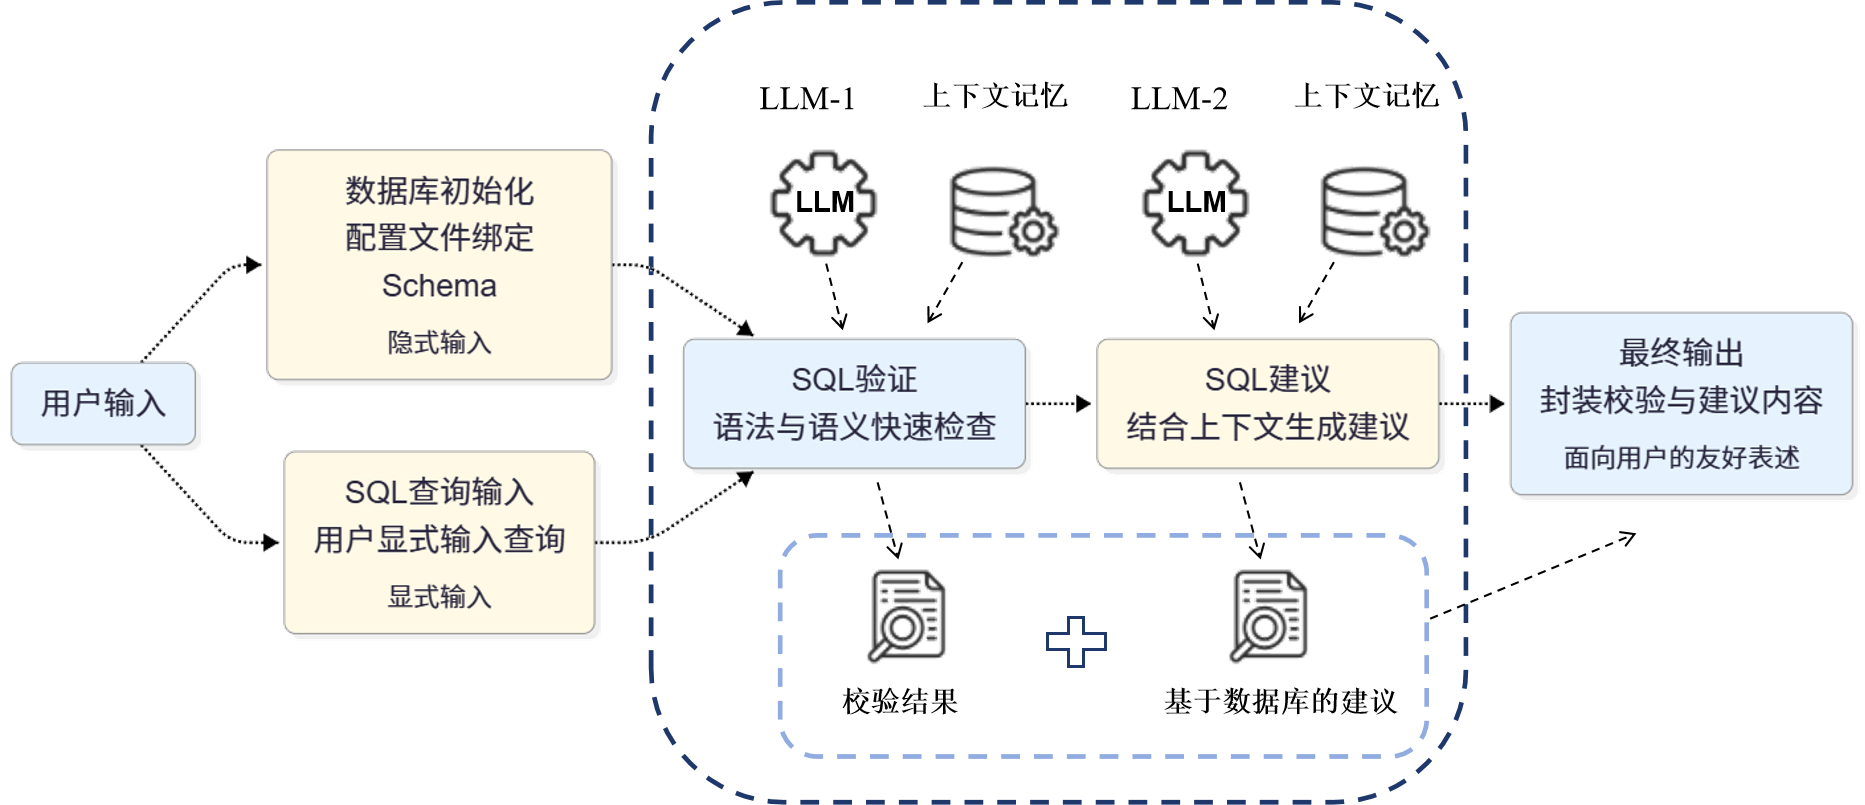
\includegraphics[width=\textwidth]{article/design/figures/workflow}
  \caption{工作流设计}
  \label{fig:agent}

\end{figure*}

Agent的优势在于可以根据实际情况自主规划和执行任务,与任务本身的贴合度高且十分灵活。但为了保证验证过程的可控性与确定性,我们设计了一个简单的工作流来约束SQL验证的主要路径,它同时接受用户的两种输入——显式输入的用户SQL查询,以及隐式加载的数据库Schema,后者在数据库初始化阶段已与配置文件绑定,无需用户再次提供。工作流的最终产出是包含语法语义结构检查、并结合性能与上下文考量的综合结果。其工作流示意图如下。

具体而言,我们注意到SQL验证工具可能存在解释不清、用户不友好问题,因此将SQL验证与SQL建议分为先后的两个任务节点。

SQL验证节点调用用户的SQL输入和数据库schema,执行快速验证,包含语法和语义的检查,返回一个初步的校验结果和对话记忆。SQL建议节点扮演资深数据库工程师与技术导师的角色。它以验证节点的校验结果与诊断上下文为输入,生成具有深度和广度的扩展性建议,运用更贴近工程实践、易于理解的语言,将初步的校验结果与扩展建议重新组织与阐释。最终输出节点将验证和建议的内容总结,打包成完整的验证结果输出。

\textbf{(2)Prompt}

我们的 SQL 验证器遵循简洁高效的提示 (Prompt) 设计策略,并参照工程化的、步骤化的思维链进行设计与部署。我们为智能体设定的角色是“资深SQL及软件工程专家”,角色的任务是接收用户输入,并调用预定义的工作流,对SQL语句进行深度验证,目标是识别并修正语法和语义层面的错误,并提供具有实践价值和用户友好的优化建议,从而全面提升SQL查询的质量。

我们设计了如下三阶段的思维链来拆解SQL验证任务,并将其固化在系统提示词中。

\textbf{1)意图识别与输入解析}

第一阶段负责对用户的原始输入进行标准化处理,以提取出待验证的目标SQL。我们要求该过程遵循以下三条规则:

纯净SQL处理:当输入为不包含任何非SQL字符的纯净SQL语句时,直接将其作为目标输入。

混合输入处理:当输入为自然语言与SQL的混合体时,系统自动提取其中的SQL部分。一个关键的例外是,若自然语言部分包含明确的文本到SQL(Text2SQL)转换意图的指令(例如,“将‘查询所有员工姓名’转换为SQL”),则优先执行转换任务,并将生成的SQL作为目标输入。

输入保真性原则:为保证验证的原始性和准确性,除上述Text2SQL的例外情况外,系统被严格禁止对提取出的SQL进行任何形式的预处理或自动纠错,必须保持其用户输入时的原貌。

\textbf{2)工作流调用与基础验证}

第二阶段是智能体执行分析任务的关键环节,我们要求智能体分三个步骤进行:

工作流启动:将阶段一解析得到的目标SQL语句sql\_input,连同通过配置文件隐式加载的数据库模式db\_info,作为参数调用预设的内部验证工作流。

语义一致性校验:在验证过程中,强制要求对SQL语句中涉及的所有数据库对象与db\_info提供的模式信息进行比对,这是确保语义正确性的关键步骤。

错误诊断与修正生成:若工作流识别出错误,智能体需生成一个或多个修正方案。当存在多种可能性时,模型被要求评估并筛选出最具工程实践价值的几种方案。若未发现错误,则直接确认原始SQL的有效性。

\textbf{3)结果整理与输出}

阶段三将分析结果以一种对用户友好且高度结构化的方式呈现,我们设计了严格的输出格式来约束:

约束性输出格式:最终响应的主体内容是SQL代码。所有的解释、说明、错误提示或优化建议,需要与代码在位置上区分开。

结果呈现逻辑:

① 对于无错误的SQL或仅有单一最优修正建议的场景,输出该条完整的SQL语句。

② 对于存在多个高价值修正建议的场景,则以带编号的列表形式呈现,每条建议后附带其完整的SQL实现,最多展示5种,为用户提供多维度的优化视角。


\end{CJK*}